\section{Results II: Reliability, Uncertainty, and Hotspot Use}

\subsection{City coverage and uncertainty outputs}

The uncertainty-aware inference package covers Almaty, Astana, Semey, and Shymkent. By construction, the calibrated median surface sums to the official total in every city. What varies is the uncertainty burden and confidence structure. Almaty has the lowest median relative uncertainty (0.170) and the largest high-confidence share (22.9\%). Semey has the highest median relative uncertainty (0.349) but still retains a small high-confidence subset (3.4\%). Astana and Shymkent are more caution-heavy and retain no high-confidence share in the reference city summary.

This city contrast is the first hint that Stage 2 is doing real interpretive work. The same calibrated proxy framework behaves differently depending on support conditions, and that difference is precisely what the uncertainty layer is designed to expose.

\begin{table}[H]
\centering
\small
\caption{Uncertainty-aware city coverage summary. The calibrated median surface sums to the official total in every city by construction. Confidence shares are reported as percentages of city cells.}
\label{tab:uncertainty-city-coverage-unified}
\begin{tabular}{lrrrrrrl}
\toprule
City & Cells & Official total & Median rel.\ unc. & High (\%) & Medium (\%) & Low (\%) & OSM label \\
\midrule
Almaty   & 3078 & 2351424 & 0.170 & 22.9 & 66.2 & 10.9 & good \\
Astana   & 3473 & 1649242 & 0.281 & 0.0  & 63.7 & 36.3 & moderate \\
Semey    & 1033 & 315382  & 0.349 & 3.4  & 79.7 & 16.9 & good \\
Shymkent & 4939 & 1298279 & 0.175 & 0.0  & 69.9 & 30.1 & moderate \\
\bottomrule
\end{tabular}
\end{table}



\begin{figure}[H]
\centering
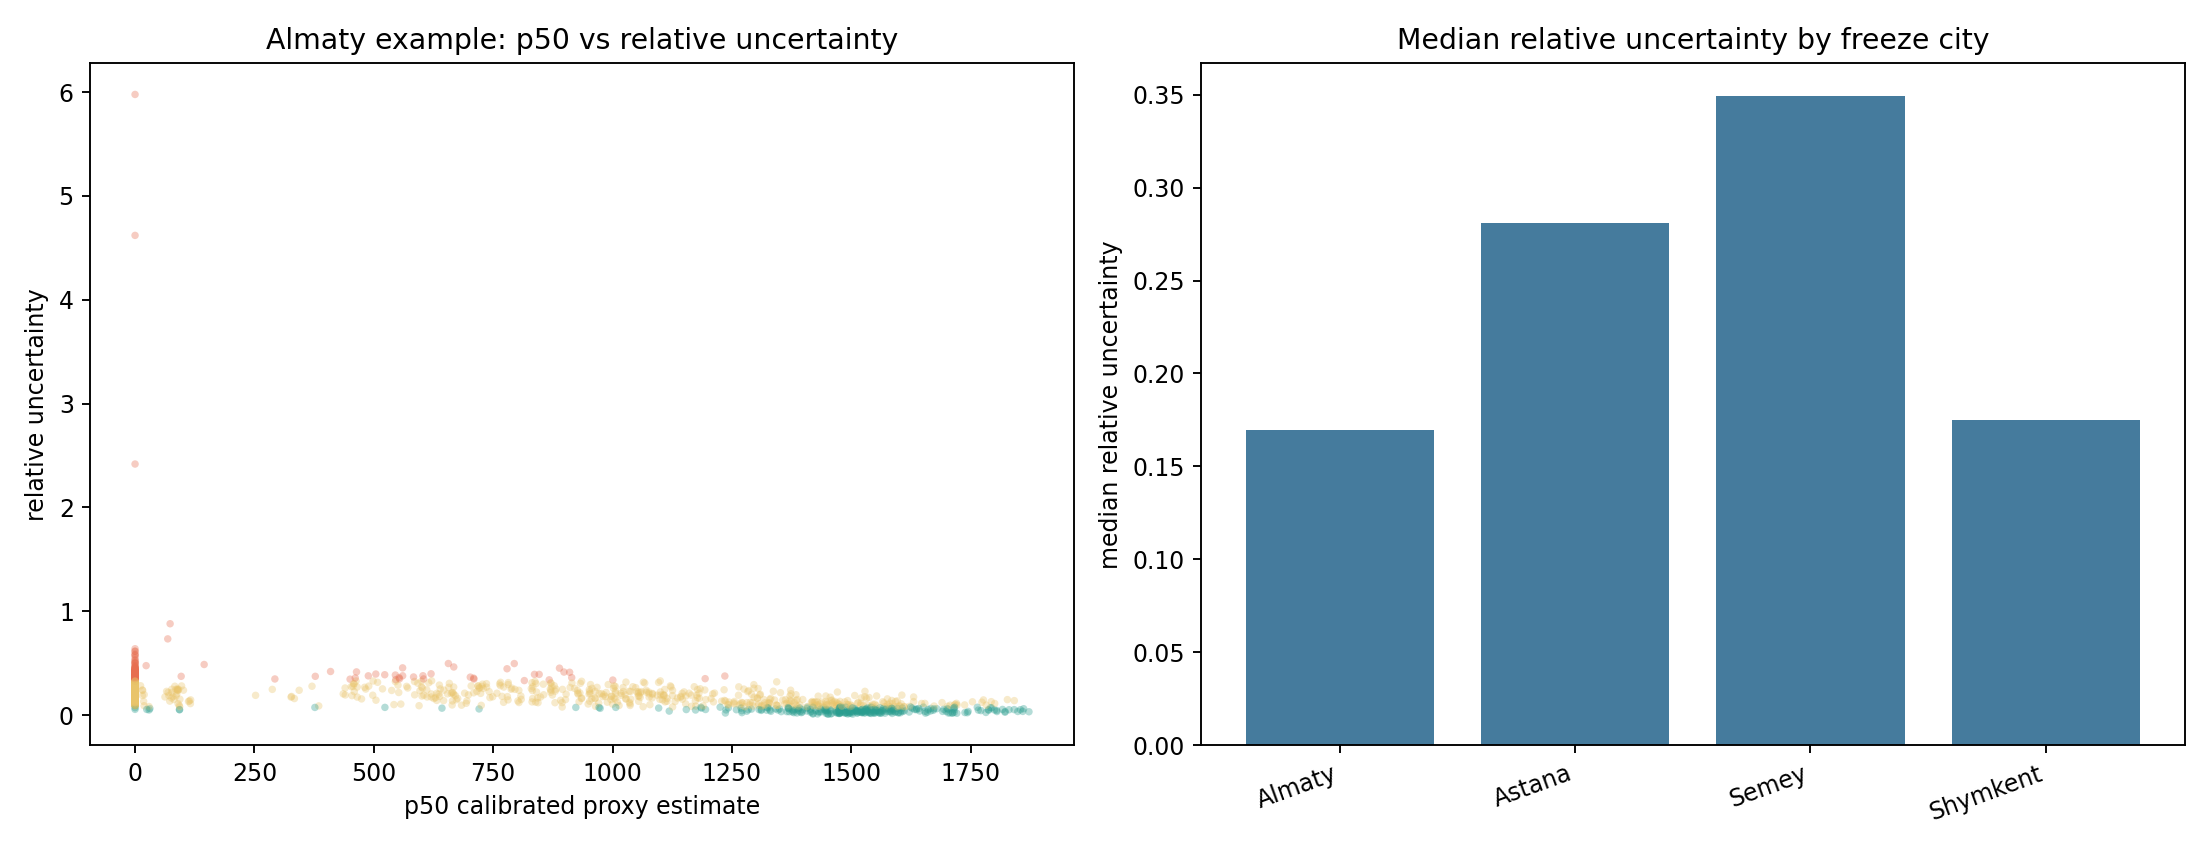
\includegraphics[width=\textwidth]{figures/fig2_uncertainty_output_example.png}
\caption{Uncertainty output summary. Left: Almaty calibrated median proxy estimates against relative uncertainty. Right: median relative uncertainty by city. The figure shows that uncertainty burden varies within and across cities, but it does not estimate true census uncertainty.}
\label{fig:uncertainty-output-unified}
\end{figure}

\subsection{Confidence-band distribution}

Confidence bands separate stronger and weaker interpretation contexts across the four-city package. Almaty is the clearest high-confidence case. Semey retains only a small high-confidence share. Astana and Shymkent are dominated by medium and low bands. These bands are interpretation support classes, not correctness probabilities.

The band separation is useful because it allows the same surface to be read differently in different cities without pretending that one summary number applies everywhere. This is the practical value of the confidence layer: it changes how the map should be used, even when the underlying median surface is unchanged.

\begin{figure}[H]
\centering
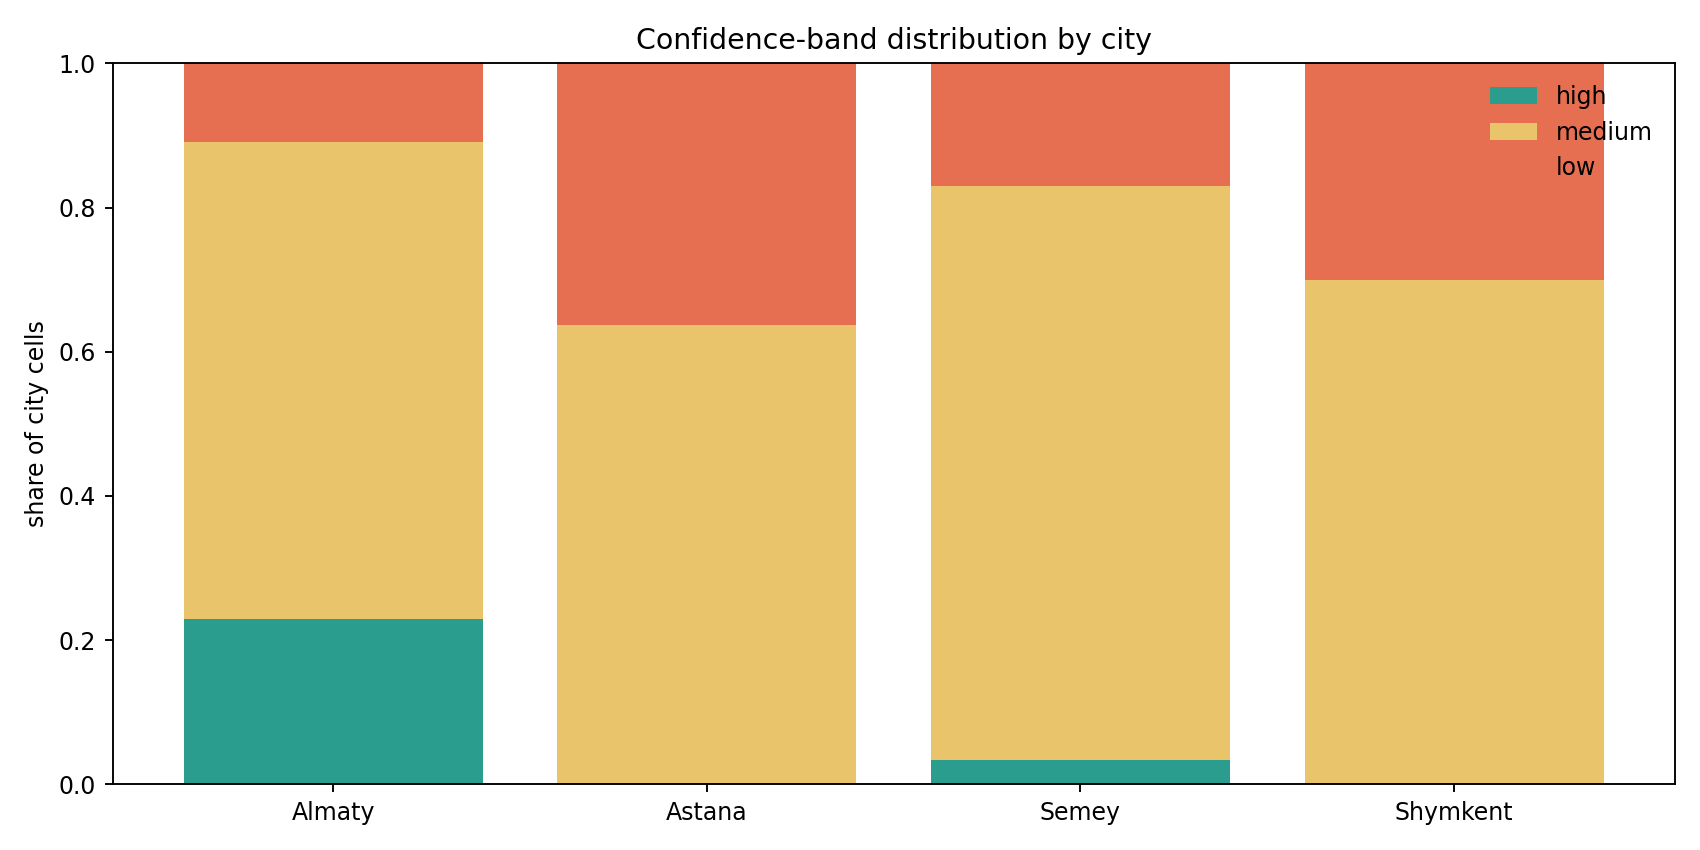
\includegraphics[width=0.95\textwidth]{figures/fig3_confidence_band_distribution.png}
\caption{Confidence-band distribution by city. The figure highlights where the calibrated proxy surface can be read more assertively for screening and where it should be treated more cautiously.}
\label{fig:confidence-distribution-unified}
\end{figure}

\subsection{Hotspot prioritization}

Hotspot prioritization translates the uncertainty layer into a bounded practical use case. Almaty is the strongest stable hotspot-screening case, with 212 \texttt{high\_value\_high\_confidence} cells and 310 \texttt{medium\_value\_high\_confidence} cells. Semey is mixed, retaining a small stable high-value subset but also a larger caution-heavy tail. Astana and Shymkent are dominated by review-oriented classes.

This is the clearest applied output of Stage 2. The framework is not saying that these are verified hotspots. It is saying that some hotspots are better supported for screening and triage than others, which is exactly the kind of distinction planners and analysts need when the evidence base is incomplete.

\begin{table}[H]
\centering
\small
\setlength{\tabcolsep}{4pt}
\renewcommand{\arraystretch}{1.08}
\caption{Hotspot prioritization summary by city. Stable high-value classes are concentrated in Almaty, whereas Astana and Shymkent are dominated by review-oriented classes.}
\label{tab:hotspot-priority-unified}
\resizebox{\textwidth}{!}{%
\begin{tabular}{lrrrrrrr}
\toprule
City & Priority cells & High/high & High/low & Medium/high & Low/high-unc. & Mean conf. & Median rel.\ unc. \\
\midrule
Almaty   & 842  & 212 & 0  & 310 & 320  & 0.609 & 0.060 \\
Astana   & 712  & 0   & 4  & 0   & 708  & 0.328 & 0.423 \\
Semey    & 169  & 4   & 19 & 10  & 136  & 0.397 & 0.591 \\
Shymkent & 1256 & 0   & 89 & 0   & 1167 & 0.323 & 0.312 \\
\bottomrule
\end{tabular}
}
\end{table}


\begin{figure}[H]
\centering
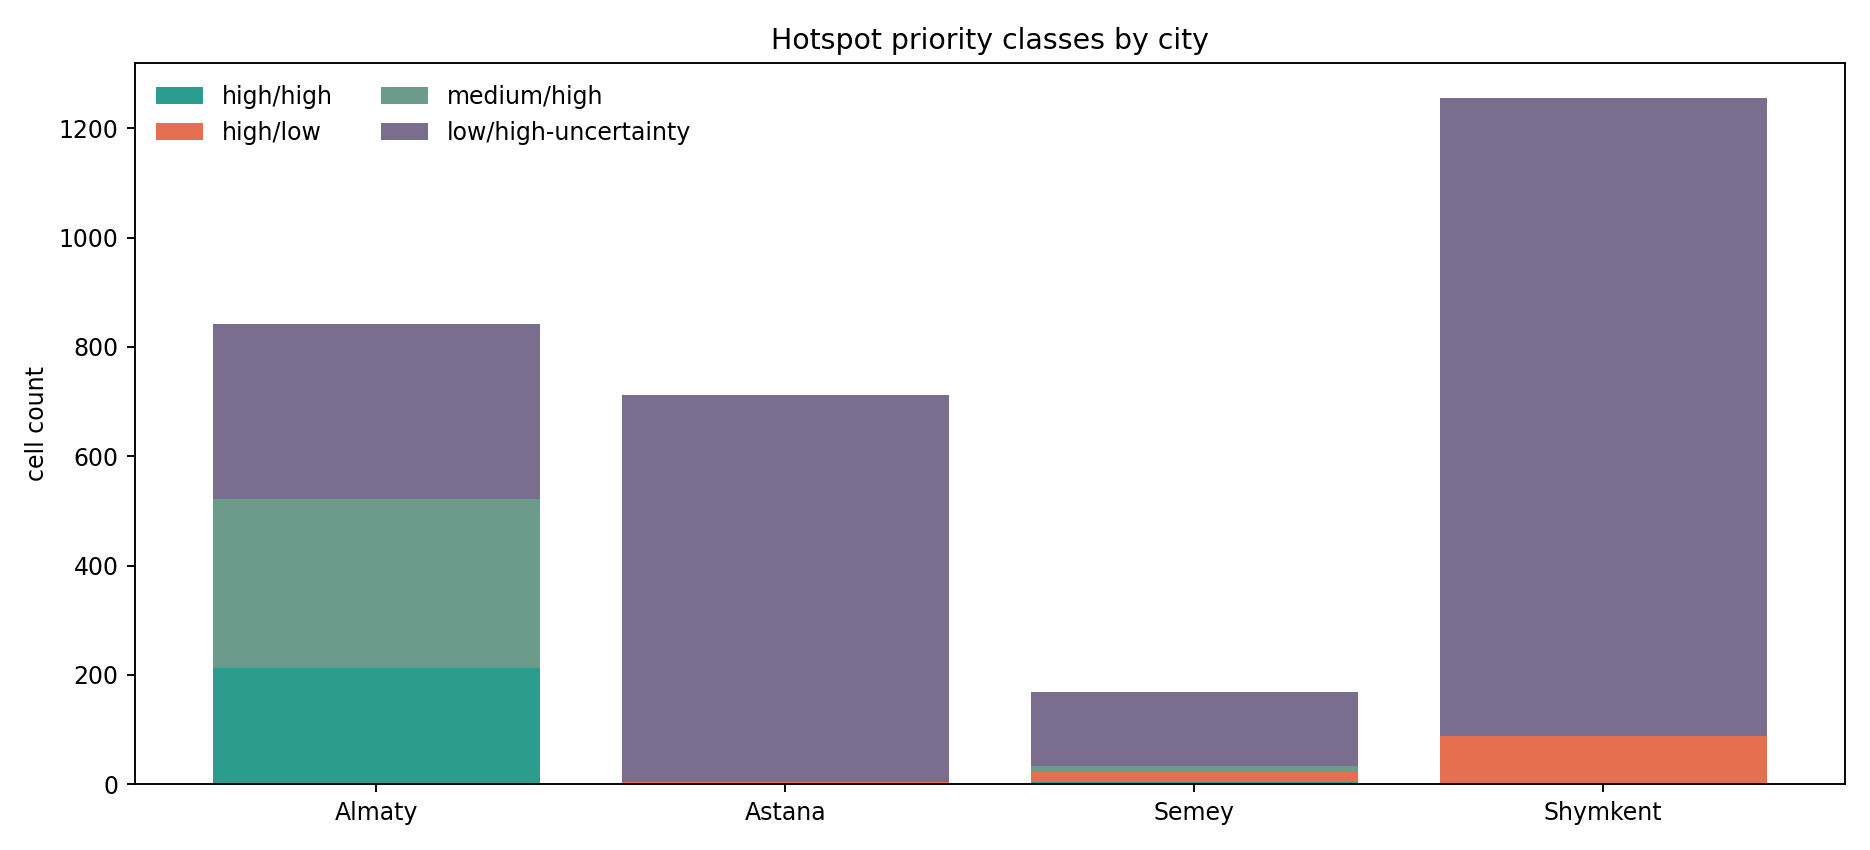
\includegraphics[width=0.95\textwidth]{figures/fig4_hotspot_prioritization_by_city.png}
\caption{Hotspot priority classes by city. Almaty concentrates the strongest stable hotspot support, whereas Astana and Shymkent are dominated by caution-oriented classes. These are screening classes rather than verified hotspot truth.}
\label{fig:hotspot-priority-unified}
\end{figure}

\subsection{Interval coverage and error alignment}

Interval coverage is mixed rather than uniformly strong. Under the bounded LOCO-like protocol, coverage ranges from 0.294 in Shymkent to 0.403 in Semey. Under the inference-only proxy check, it improves to 0.598 in Almaty, 0.613 in Astana, 0.692 in Semey, and 0.534 in Shymkent. This supports bounded interval usefulness, not full uncertainty calibration.

The mixed coverage result is important because it keeps the paper honest. It shows that the ensemble spread is informative, but not enough on its own to justify a claim of fully calibrated uncertainty. This is why coverage remains secondary evidence rather than headline evidence.

\input{tables_tex/table9_interval_coverage_summary.tex}

Uncertainty width tracks proxy-target error positively across all retained city/protocol combinations, with Spearman correlations between 0.689 and 0.886. By contrast, relative-uncertainty ordering and confidence ordering remain mixed, so the broader confidence-error story should be stated cautiously.

That mixed ordering is not a failure; it is a boundary condition. It tells us that the width signal is meaningfully aligned with error, but the rest of the confidence hierarchy is not uniformly monotonic. The manuscript should therefore claim directional usefulness, not perfect calibration.

\begin{table}[H]
\centering
\scriptsize
\caption{Error-uncertainty alignment summary. Positive width-error correlations are retained across all shown city/protocol combinations, whereas relative-uncertainty and confidence ordering remain mixed.}
\label{tab:error-alignment-unified}
\begin{tabular}{p{2.4cm}p{1.4cm}rrrr}
\toprule
Protocol & City & \shortstack{Spearman\\(error, width)} & \shortstack{Pearson\\(error, width)} & \shortstack{Spearman\\(error, rel.\ unc.)} & \shortstack{Spearman\\(error, confidence)} \\
\midrule
LOCO-like & Almaty   & 0.713 & 0.384 & -0.449 & 0.448 \\
LOCO-like & Astana   & 0.759 & 0.541 & -0.220 & 0.221 \\
LOCO-like & Semey    & 0.743 & 0.493 & -0.354 & 0.354 \\
LOCO-like & Shymkent & 0.689 & 0.535 & -0.387 & 0.387 \\
Inference-only proxy & Almaty   & 0.749 & 0.657 & -0.347 & 0.346 \\
Inference-only proxy & Astana   & 0.777 & 0.616 & -0.042 & 0.042 \\
Inference-only proxy & Semey    & 0.752 & 0.602 & -0.337 & 0.333 \\
Inference-only proxy & Shymkent & 0.886 & 0.826 & -0.421 & 0.421 \\
\bottomrule
\end{tabular}
\end{table}



\begin{figure}[H]
\centering
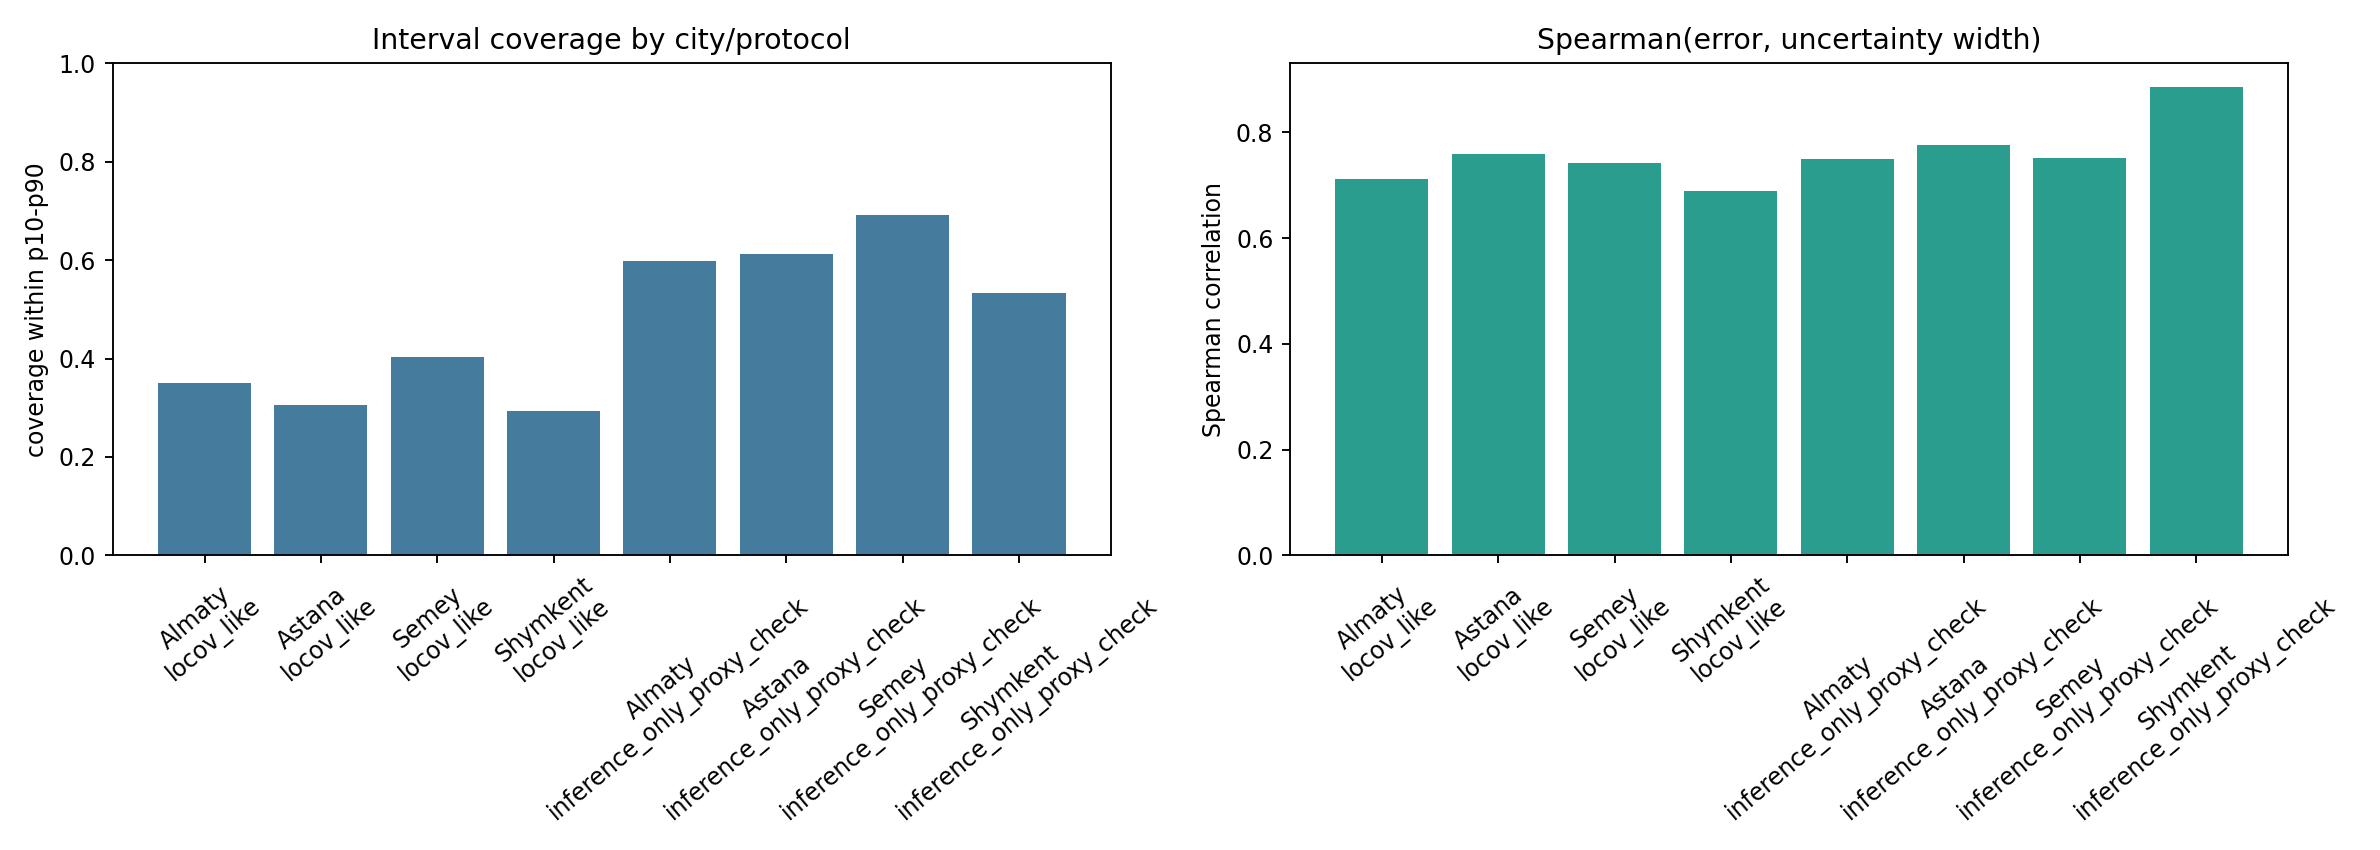
\includegraphics[width=\textwidth]{figures/fig5_uncertainty_validation_summary.png}
\caption{Summary of interval coverage and error-width alignment. Coverage is mixed across protocols, but uncertainty width carries meaningful positive alignment with proxy-target error.}
\label{fig:uncertainty-validation-unified}
\end{figure}

\subsection{Confidence bands and hotspot stability}

Where a high confidence band exists, it shows lower relative uncertainty than the low band. Almaty provides the clearest separation, from 0.044 in the high band to 0.396 in the low band. Semey also shows strong separation, from 0.061 to 0.593, despite its more mixed overall screening position.

This is the cleanest confidence-band argument in the paper. It shows that the banding scheme is not decorative: it actually sorts cells by support level in a way that can be used for screening and prioritization.

\input{tables_tex/table11_confidence_band_summary.tex}

Hotspot stability is the strongest uncertainty evidence layer. Stable classes such as \texttt{high\_value\_high\_confidence} and \texttt{medium\_value\_high\_confidence} retain much higher mean stability metrics than caution-heavy classes. This is the clearest evidence that the uncertainty-aware stage does useful screening work rather than merely adding decorative interval columns.

That makes hotspot stability the main Stage 2 takeaway. If a reviewer asks what the uncertainty layer actually adds, the answer is not "more numbers"; it is that the layer distinguishes stable screening candidates from review-heavy ones in a way that is internally coherent across the ensemble.

\begin{table}[H]
\centering
\small
\caption{Hotspot stability summary by class. Stable classes retain substantially higher mean stability metrics than caution-heavy classes across the four-city inference package.}
\label{tab:hotspot-stability-unified}
\begin{tabular}{lp{2.8cm}rrrr}
\toprule
City & Hotspot class & Cells & Mean stability & Median rel.\ unc. & Mean confidence \\
\midrule
Almaty   & high/high      & 212  & 0.777 & 0.044 & 0.738 \\
Almaty   & medium/high    & 310  & 0.784 & 0.037 & 0.745 \\
Almaty   & low/high-unc.  & 320  & 0.263 & 0.398 & 0.391 \\
Astana   & high/low       & 4    & 0.219 & 0.369 & 0.354 \\
Astana   & low/high-unc.  & 708  & 0.176 & 0.423 & 0.328 \\
Semey    & high/high      & 4    & 0.834 & 0.076 & 0.711 \\
Semey    & medium/high    & 10   & 0.825 & 0.065 & 0.717 \\
Semey    & high/low       & 19   & 0.197 & 0.590 & 0.369 \\
Semey    & low/high-unc.  & 136  & 0.292 & 0.603 & 0.369 \\
Shymkent & high/low       & 89   & 0.225 & 0.272 & 0.354 \\
Shymkent & low/high-unc.  & 1167 & 0.200 & 0.317 & 0.321 \\
\bottomrule
\end{tabular}
\end{table}



\begin{figure}[H]
\centering
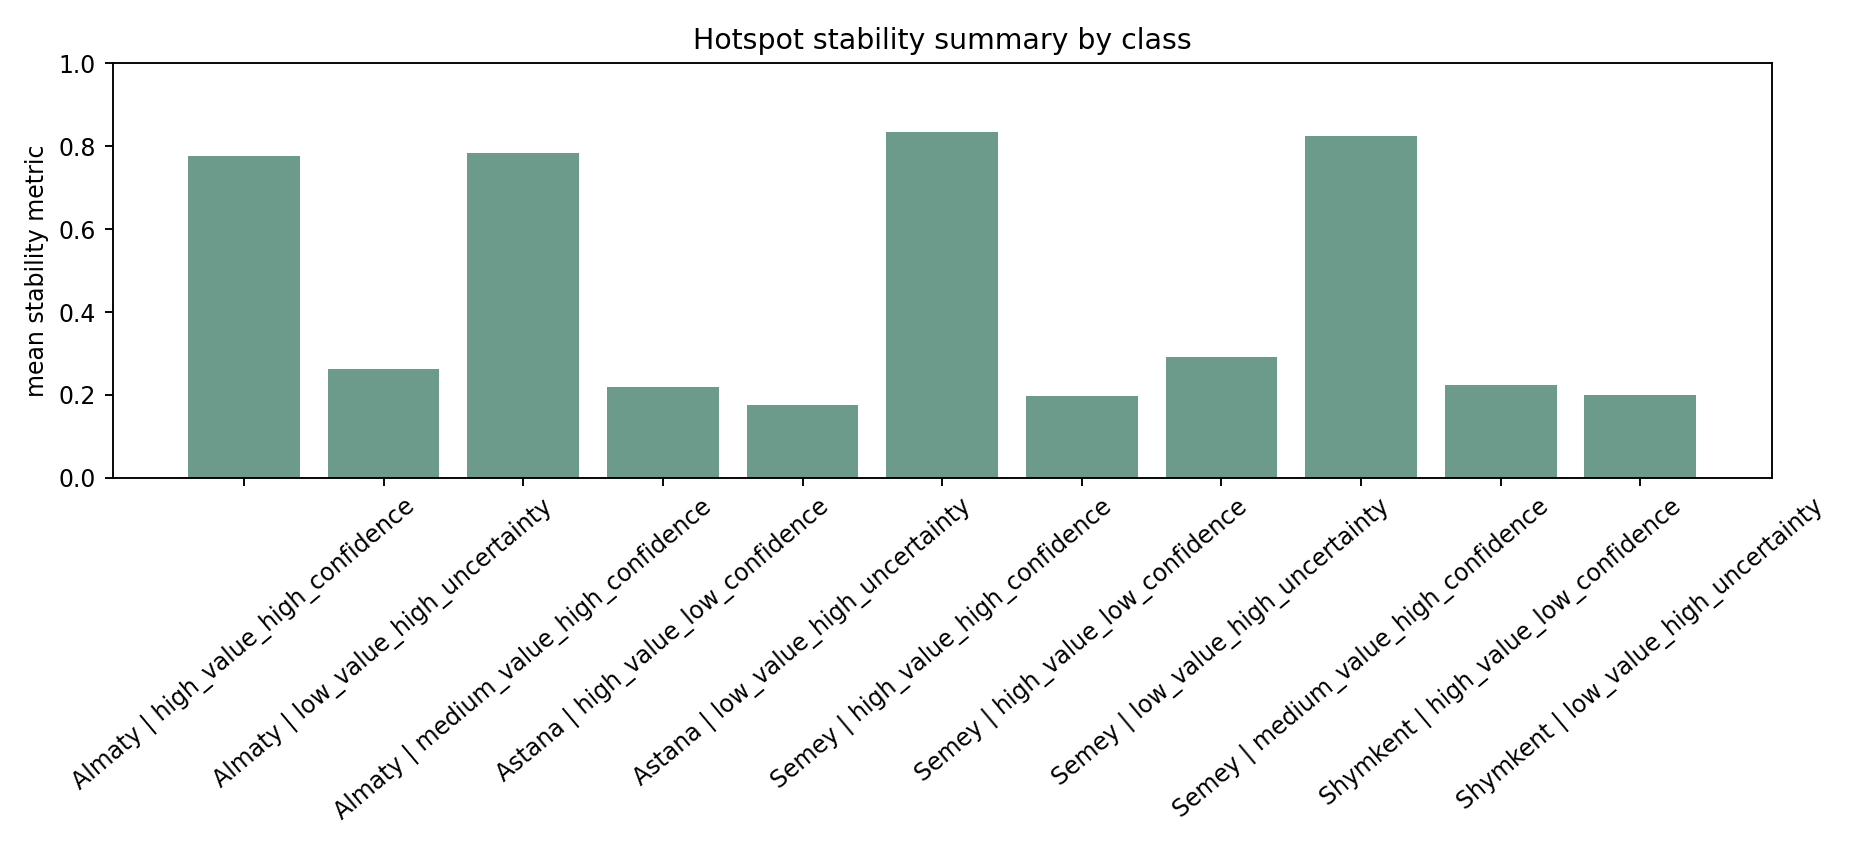
\includegraphics[width=\textwidth]{figures/fig6_hotspot_stability_summary.png}
\caption{Hotspot stability summary by class. Stable classes retain much higher mean stability than caution-heavy classes, making hotspot stability the strongest evidence layer for the uncertainty-aware stage.}
\label{fig:hotspot-stability-unified}
\end{figure}

\subsection{District and external uncertainty evidence}

The remaining uncertainty evidence layers are informative mainly as limitations. District interval coverage remains partial because true district p10/p50/p90 testing is blocked by missing district polygon/cell assignment artifacts in the light package. External disagreement alignment against WorldPop and GHS-POP is mixed or negative, so the data do not support a strong claim that uncertainty rises systematically where external disagreement increases.

These weaker layers do not invalidate Stage 2. They simply constrain it. They tell the reader that the uncertainty layer is best understood as a screening and interpretation layer, not as a full probabilistic truth model.

\begin{table}[H]
\centering
\scriptsize
\caption{District and external uncertainty evidence retained in the reference package. These layers are informative mainly as context and limitation evidence rather than as strong validation support.}
\label{tab:district-external-uncertainty-unified}
\begin{tabular}{p{2.6cm}p{2.2cm}p{1.2cm}p{3.1cm}p{5.1cm}}
\toprule
Evidence layer & Scope & Status & Available result & Limitation for interpretation \\
\midrule
District interval coverage & Almaty & partial & compared = 6; mean abs.\ error p50 = 94209.1 & True district p10/p50/p90 coverage remains blocked because frozen district polygon/cell assignments are missing. \\
District interval coverage & Astana & partial & compared = 5; mean abs.\ error p50 = 169626.3 & Treat only as partial administrative support after aggregation. \\
District interval coverage & Shymkent & partial & compared = 3; mean abs.\ error p50 = 108862.2 & Does not provide district interval validation or cell-level truth. \\
External disagreement alignment & Almaty / WorldPop & mixed & Spearman(disagreement, uncertainty) = -0.299 & External products provide structural comparison context, not ground truth. \\
External disagreement alignment & Almaty / GHS-POP & mixed & Spearman(disagreement, uncertainty) = -0.494 & Mixed or negative alignment does not support strong monotonicity claims. \\
External disagreement alignment & Astana / WorldPop & mixed & Spearman(disagreement, uncertainty) = -0.188 & Structural benchmark only. \\
External disagreement alignment & Astana / GHS-POP & mixed & Spearman(disagreement, uncertainty) = -0.251 & Structural benchmark only. \\
External disagreement alignment & Shymkent / WorldPop & mixed & Spearman(disagreement, uncertainty) = -0.422 & Structural benchmark only. \\
External disagreement alignment & Shymkent / GHS-POP & mixed & Spearman(disagreement, uncertainty) = -0.451 & Structural benchmark only. \\
\bottomrule
\end{tabular}
\end{table}



These are limitations, not fatal flaws. They narrow the claim boundary of the uncertainty-aware stage and reinforce that the correct interpretation is screening reliability rather than true uncertainty calibration.
